\documentclass{article}
\usepackage[top=1.5cm,right=3cm,bottom=2cm,left=1.5cm]{geometry}

\usepackage[T1]{fontenc} \usepackage[utf8]{inputenc}
\usepackage{authblk}
\usepackage{graphicx} 
\usepackage{hyperref}
\usepackage{amsmath}\usepackage{amsfonts}
\newcommand{\deq}{\stackrel {\rm def}{=}}
\newcommand{\eqline}[1]{\\\centerline{$#1$}\\} 
\newcommand{\hr}{\\---------------------------------------------------}
\newcommand{\tab}{\\\hspace{5mm}} 

\begin{document}

\title{Adjusting meta-parameter in machine learning}
\author{@anthony ? @fred ? @thalita ? @xavier ?}

\section{Introduction}

Automated machine learning\footnote{The notions of ``\href{https://en.wikipedia.org/wiki/Automated\_machine\_learning}{automated-machine-learning}'', 
``\href{https://en.wikipedia.org/wiki/Meta_learning_(computer_science)}{meta-learning}'', including ``\href{https://en.wikipedia.org/wiki/Meta-optimization}{meta-optimization}'' and ``\href{https://en.wikipedia.org/wiki/Hyperparameter_(machine_learning)}{hyper-parameter}'' and the related ``\href{http://neupy.com/2016/12/17/hyperparameter\_optimization\_for\_neural\_networks.html}{hyper-parameter optimization}'', have precise meaning in machine-learning, and we assume this is known to the reader.} is ``the process of automating the end-to-end process of machine learning'', because the complexity of adjusting the hyper-parameters, including selecting a suitable method, becomes easily time-consuming when not intractable. To this end, the general idea is to consider a standard machine-learning algorithm and to add on ``top of it'' another algorithmic mechanism, e.g., another machine learning algorithm dedicated to automatic hyper-parameter adjustment, with the caveat of generating other hyper-parameters for the meta-learning algorithm and without formal guaranty that this accumulation of mechanisms is optimal.

Here we propose to follow another track: To what extent could hyper-parameters be integrated as algorithm parameters ? In other words : How is it possible to consider the automatic adjustment of hyper-parameters not as a separate process but within the learning algorithm itself ? Let us call such parameters {\em meta-parameters} and let us attempt to formalize such an alternative track.

\paragraph{Related work.} {\tt @todo : demander à  @anthony @fred @thalita @xavier leurs key-papers pour faire ce paragraphe}.

\section{Meta-parameter adjustment set-up}

\paragraph{Problem position.}

We consider the estimation problem of parameters ${\bf w}$, by the optimization of a criterion $c(\dot)$, using an algorithm of, say minimization, ${\cal A}$. This algorithm is parameterized by meta-parameters ${\bf \theta}$. It is applied on the criterion $c(\dot)$, for some initial values ${\bf w}_0$:
\eqline{{\bf w} = \mbox{arg max}_{\bf w} c({\bf w}) \;\;\;\left\backslash \;\;\; {}_{\bf \theta}{\cal A}\left(c, {\bf w}_0\right). \right.}

Without loss of generality for our purpose we consider that the algorithm writes: 

{\tt ~
\\\indent ${\cal A}_{\mbox{initialize}}(c, {\bf w} = {\bf w}_0)$
\\\indent do \{
\\\indent \indent ${}_{\bf \theta}{\cal A}_{\mbox{run-one-step}}(c, {\bf w})$
\\\indent \indent ${\cal A}_{\mbox{adjust meta-parameters}}({\bf \theta})$
\\\indent \} until(${\cal A}_{\mbox{has-converged}}(c, {\bf w})$)
\\
}

The goal here is to design the ${\cal A}_{\mbox{adjust meta-parameters}}({\bf \theta})$ mechanism. This algorithmic construct is general, since nested loops can almost always be rewritten in terms of a unique loop\footnote{For instance the construct:
\\\indent {\tt do \{ do \{ learning-step() \} until(ok1()); hyper-parameter-adjustment(); \} until(ok2());\}}
\\rewrites, e.g.:
\\\indent {\tt do \{ learning-step(); b = ok1(); if (b) \{ hyper-parameter-adjustment(); \} \} until(b and ok2());\}}
\\ See \cite{collard2007reasoning} for a more general discussion.}. Furthermore, to develop our method, we do not need more details about the criterion and the optimization algorithm, but on the meta-parameters specification. 

\paragraph{Meta-parameter specification.}

More precisely, we consider that a meta-parameter has either a qualitative value, i.e., a finite enumeration of values, or a quantitative value. In this latter case such value is bounded with finite precision, i.e., has {\tt minimal} and {\tt maximal} values, a {\tt default} value and a {\tt precision} below which two values are indistinguishable (see Appendix~\ref{about-quantitative-values}). We further often observe \cite{} that only a small set of values are sufficient to optimize the meta-parameters. 

For instance considering a standard back-propagation algorithm which samples some data batches of a given {\tt batch-size} and apply on such batches {\tt epoch-duration} iterations of a 1st order minimization parameterized by a given {\tt learning-rate}, with a option regarding a specific algorithmic variant (here {\tt desired-value} hidden unit prediction from the provided output values, as discussed in \cite{vieville:hal-01610735}) we may write:{\small \begin{verbatim}
  {
    batch-size       : [1, 2, 5, 10, 20 , 50, 100, 200],
    epoch-duration   : [1, 5, 10, 15, 20, 25],
    learning-rate    : { min : 1e-12, max: 1, step: 1e-6, default: 1 },
    desired-value    : {false, true}
  }
\end{verbatim}}
\noindent where the {\tt batch-size} is enumerated as a logarithmic quantity, the {\tt epoch-duration} as a linear quantity, the {\tt learning-rate} as a quantitative parameter, and the {\tt desired-value} option as a Boolean. In this framework, non-numeric values can either be considered as sorted values (e.g. {\tt ['false', 'undefined', 'true']}, i.e. isomorphic to {\tt [0, 1, 2]}) or unsorted values (e.g. {\tt \{false, true\}}).

In the sequel, both the continuous and discretized nature of the meta-parameter set is going to be used. We note $p_i$ the value of the parameter of index $i$ and $p_{ij}$ its $j$-th discretized value.

At the implementation level, we observe \cite{} an order of magnitude of 1000 values, i.e., 100 values for 10 meta-parameters. The algorithmic complexity will in any case be linear be linear with this number of values, thus able to scale to a higher order of magnitude, if needed.

\paragraph{Meta-parameter adjustment.}

Some parameters are expected to be ``observable in one step'' in the sense that their value is going to mainly influence the next ${}_{\bf \theta}{\cal A}_{\mbox{run-one-step}}(c, {\bf w})$ algorithm step. This is the case for the learning-rate.

This is however not the case of most parameters. Considering, e.g., deep networks, meta-parameters include structural parameters (such as the number of layers, and within a layer the number of units (hidden units and output units), the unit connection size (e.g. convolution layer filter size) and/or form, the choice of the non-linearity (i.e., of the activation function), the choice of the loss function and the parameters of the regularization part of such loss function, or the parameter initialization method. The effect of all these values can not be observed from one step to another, but considering a whole epoch (i.e., a training cycle on the training set). This the case of the batch-size and epoch-duration in our example. 

Yet another step further, if the parameter initialization method is not deterministic (e.g., using transfer learning from another data set) but based on resetting the weights from different random draws in order to explore several solutions (i.e., in the presence of local minima), then the observation is not limited to one epoch but a bench of epochs. Our discussion must now apply on epoch of epochs.

Such meta-parameter observation time is now a meta-meta-parameter. There are different ways to take into account such epoch observation: one is to run the optimization until convergence and observe the final result, which means that the meta-parameter defining what is the convergence is now a meta-meta-parameter, while we have to accept long calculation times. Another option is to run the optimization during a fixed period of time (i.e., the epoch-duration) considering that we want to observe the best gain in accuracy for a given number of steps, which now means that the observation itself is influenced by a meta-parameter to observe. A chicken-and-egg problem.

Here we are going to develop a third solution, which is to introduce an additional knowledge. We consider the criterion decay in order to predict, without having to run the criterion up to convergence, the final criterion value interpolation, as soon as available. The implementation of this idea is detailed in Appendix~\ref{about-decay-fit} and it is an example of parameter-less mechanism.

\paragraph{Choosing a performance indicator.}

Given the criterion cost $c(t) > 0$, the following performance indicator is considered, given costs $c(t)$ at time $T(t)$:
\eqline{{}_T\delta_c(t) \deq \delta_c(t) \, \frac{1}{T(t) - T(t-1)}, \;\;\; \delta_c(t) \deq \max\left(\frac{-c(t) + c(t-1)}{c(t-1)}, 0\right)}
in words the relative cost decrease speed. The cost is obtained after one step, in the ``observable in one step'' case. Otherwise, it is observed after a criterion final value prediction.

Depending on the application, the time $T(t)$ corresponds to the iteration index (i.e., $T(t) = t$, so that ${}_T\delta_c(t) = \delta_c(t)$), the processor CPU time if the computation time is to be taken into account, or the system real time if the algorithm is embedded in a more complex system.

The criterion decrease $\delta_c(t) \in [0, 1]$, where the lower value $0$ corresponds to the fact that the algorithmic step yields no improvement, whereas the higher value $1$ corresponds to the fact that $c(t) = 0$, i.e., the problem has an exact solution, found in one step.

Clearly the goal is to obtain meta-parameters such that the ${}_T\delta_c(t)$ is maximal. However, such a value is not deterministic. We thus will specify the goal {\em obtaining a ${}_T\delta_c(t)$ distribution with the highest mean}. Furthermore, we observe \cite{} that for good meta parameters $\delta_c(t)$ is randomly distributed in $[0, 1]$, i.e., the goal is {\em not having ${}_T\delta_c(t)$ always $0$}. In other words, we accept the fact that a meta-parameter value may yield a small criterion decrease, providing that this is a seldom event. On the contrary, a bad meta-parameter value will determistically produces a small when not negligible criterion decrease. This corresponds to {\em bounded constrained maximal entropy distribution} as detailed in Appendix~\ref{bcmed}, and this formulation is the core of our method. 

Let us now consider, based on this set-up, some meta-parameter optimizer behaviors.

\section{The marginal meta-parameter optimizer}

Let us start considering a meta-parameter optimizing behavior that we often use, as a human operator. This marginal meta-parameter optimizer considers the following requirements:
\\ - We consider only a finite number of values for each meta-parameters,
\\ - We better change only one meta-parameter at a time in order to observe interpretable reaction of the algorithm,
\\ - We better choose the parameter index and parameter value that will maximize the performance indicator, but also our information our the criterion.

In order to instanciate these ideas, we calculate for each parameter value the following local and global momenta, for $d \in \{0, 1, 2\}$, at time $t$:
\eqline{\left\{\begin{array}{rcl}
 m_{d,ij} &=& \left.\sum_{s=1}^{s=t} (1 - \gamma) \, \gamma^{t-s} \, c(s)^d\right|_{p_i = p_{ij}}\\
 m_{d} &=& \sum_{s=1}^{s=t} (1 - \gamma) \, \gamma^{t-s} \, c(s)^d\\
\end{array}\right.}
the expectation being computed using the 1st-order exponential filter optimal parameter $\gamma$ estimated on the criterion decay fit as detailled in Appendix~\ref{about-decay-fit}. These momenta leads to the following estimations of :

Given these requirements, we propose to maximize the expectation comp
@todo choix du paramètre : dispersion maximale ? 

@todo ajustement modele constant versus quadratique sur parametre 

@todo sorted parameter (thus quadratic (lamda = m0 / sd$^2$) ) or not (thus random draw selom m1o)

@todo  m1o = m0 m1 + (1-m0) (m0\_all m1\_all + (1 - m0\_all) 1/2)

@todo  pemaliser selon sqrt(m2/N - m1$^2$) - sd(m) 

@todo  relier m0 à 1/N : ou N ou e m0 = gamma m0 + (1-gamma) 1 = 1 - gamma$^N$

@todo choix du parametre selon meileur m1o avec random draw 

@todo commencer par ne pas utiliser m2 sauf pour eliminer les metas parametres 

\appendix

\clearpage \section{Quantitative value specification} \label{about-quantitative-values}

In numerical algorithms a quantitative quantity $q$ is always reasonably defined within bounds $q \in [q_{\min}, q_{\max}]$, with a default value $q_0$ (the middle of the interval, if no better knowledge), and with a precision $q_\epsilon$, such that:
\eqline{|q' - q''| < q_\epsilon \;\;\Leftrightarrow\; \mbox{$q'$ and $q''$ are indistinguishable},}
while this specification can be linear or logarithmic (i.e. apply on $\log(q)$).
Such design choice has many advantages:
\\- It allows the detection of aberrant or overflown values.
\\- It allows the use of a default initial or fallback value.
\\- It allows the definition of precision threshold under which numerical refinement is useless.
\\- It defines a maximal sampling to map this continuous value on a finite data set.
\\- Such specification is useful for display or user interface.
\\ It is also important to notice that such information is always available in practice, e.g., a pupil ruler has a precision of 1mm, with bounds defined by the ruler length; a location in an image is within the image sizes with a standard precision of one pixel; a car velocity is 0 by default and bounded by the vehicle performances, while the precision is not better than 1 km/h; and so on.

Beyond this proposal is the fact that in terms of interpretability, it is more easy for a end user to provide as much relevant a-priori information as possible, than to manipulate opaque hyper-parameters.

\clearpage \section{Parameter-less exponential decay fit.} \label{about-decay-fit}

In order to design a parameter-less exponential decay fit, we consider a constant, affine or exponential triplet of models of the a time series $c(t)$ writing :
\eqline{\hat{c}(t) = \left\{\begin{array}{ll} 
 \beta                      & \mbox{constant,} \\
 \beta + \nu \, t           & \mbox{affine,} \\
 \beta + \nu \, e^{-t/\tau} & \mbox{exponential,} \\
\end{array}\right.}
in order to detect the quantitative and qualitative behaviors of the criterion evolution:
\\- If a constant model is prefered, it means that the criterion is no more decreasing, while the obtained value estimation is $\beta$.
\\- If an affine model or an exponential concave model is prefered, it means that the criterion is decreasing without any evaluation of the final value and time constant.
\\- If an exponential convex model is prefered, this provides an estimation of both the decay time-constant $\tau$ and the final value $\beta$.

The reason of this design choice is that we may encountered really non-stationnary criterion decay profiles as shown in Fig.\ref{spurious-cost}.

\begin{figure}[!ht]
\centerline{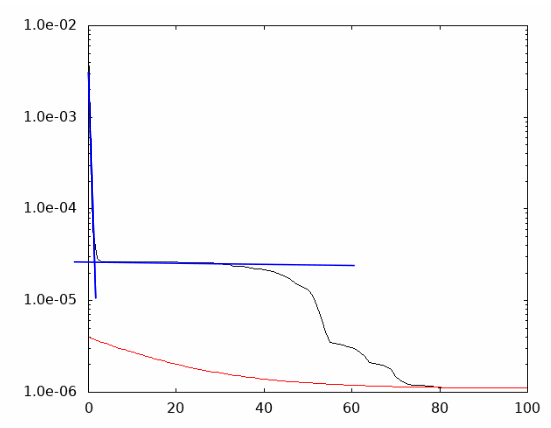
\includegraphics[width=0.8\textwidth,height=4cm]{img/spurious-cost}}
  \caption{An example of non-stationnary profile with several transitions, reproduced from \cite{vieville:hal-01610735}. In back the criterion decay $c(t)$. In blue two transient affine interpolations. In red the convex exponential interpolation, when the criterion is in convergence phase. Our experimental observation is that during such transient periods, the sliding-window criterion interpolation is more affine or concave, than convex. It is furthemore numerically important to consider several sliding-window sizes.}
  \label{spurious-cost}
\end{figure}

Since the criterion decay is not stationary, we must evaluate the models in a sliding window, which means computing any quantity $\omega$ using mainly the short-term previous values. Considering a 1st order exponential decay filter, we can use as expectation estimator:
\eqline{\mathbb{E}[\omega]_{t} = \sum_{s=1}^{s=t} (1 - \gamma) \, \gamma^{t-s} \omega_s = \gamma \, \mathbb{E}[\omega]_{t - 1} + (1 - \gamma) \, \omega_{t-1} , \, \gamma = \upsilon^{\frac{1}{w}} \in [0, 1]}
for some parameter $\gamma$ corresponding to a window size of $w$ steps, containing in proportion $1 - \upsilon$ of the filter coefficients (i.e. $\sum_{s=t-w-1}^{s=t} (1 - \gamma) \, \gamma^{t-s} = 1 - \upsilon$). 

At the numerical level for $\upsilon \in [1/1000, 1/10]$ and $w \in [8, 512]$, which seems reasonable concrete values bounds, we obtain:
\eqline{\small \begin{array}{c|cccccccc} \upsilon & w: &8&16&32&64&128&256&512\\ 
  \hline
   0.1&& 0.75& 0.87& 0.93 & 0.96& 0.98& 0.99& 0.99\\ 
  0.05&& 0.69& 0.83& 0.91& 0.95& 0.98& 0.99& 0.99\\ 
  0.02&& 0.61& 0.78& 0.88& 0.94& 0.97& 0.98& 0.99\\ 
  0.01&& 0.56& 0.75& 0.87& 0.93& 0.96& 0.98& 0.99\\ 
 0.005&& 0.52& 0.72& 0.85& 0.92& 0.96& 0.98& 0.99\\ 
 0.002&& 0.46& 0.68& 0.82& 0.91& 0.95& 0.98& 0.99\\ 
 0.001&& 0.42& 0.65& 0.81& 0.90& 0.95& 0.97& 0.99\\
\end {array}}
thus may consider $\gamma \in [0.4, 0.99] \simeq \{0.40,  0.53,  0.64,  0.73, 0.81,  0.87,  0.92,  0.96,  0.98,  0.99\}$ 
which appears here as a meta-meta-parameter. Considering only a few enumeration of values seems sufficient, since the influence of such time window is not very sensitive.

The time decay $\tau$ is estimated in the least-square sense on:
\eqline{\min_{1/\tau, k} \sum_{t}^{T-1} \gamma^{T-t} \, (k - sg(c(t) - c(t-1)) \, t / \tau - \log(|c(t) - c(t-1)|))^2,}
while the bias $\beta$ and $\nu$ gain are computed using standard similar weighted least-square criterion ($\tau$ being given in the exponential case, by the previous estimation):
\eqline{\min_{\nu, \beta} \epsilon^2, \;\;\; \epsilon^2 \deq \sum_{t}^{T-1} \gamma^{T-t} \, (c(t) - \hat{c}_{\nu, \beta|\tau}(t))^2}
for the three models. Here we consider previous values, but not the last one.

The model is chosen comparing the weighted squared-errors $\epsilon^2 / (W - D)$ of the three alternatives, where $D$ is the model number of parameters, thus using a very standard test (see, e.g., \cite{vieville:inria-00000172} for a discussion).

Then, the best model prediction is tested on the last value $c(T)$, since this sample has not been taken into account for the estimation of the parameters and mode. We thus compute the following expectation, at time $T_0$:
\eqline{\varepsilon^2 = \sum_{T=0}^{T=T_0} \gamma^{T_0-T} \,  (c(T) - \hat{c}_{|\nu,\beta,\tau}(T))^2.}
This yields a way to optimize $\gamma$, considering the value minimizing this prediction error expectation. We now have a parameter-less estimator able to learn its own hyper-parameter, transformed in meta-parameter.

At the implementation level, we propose to run in parallel the estimator for the sampled $\gamma$ values in order to select at each step-time the best one, given the model prediction error. We propose this ``brute force method'' of parallel independent channels. The amount of calculation is rather small, about 20 operations (addition or multiplication) at each step for each channel, plus less than 50 operations by channel when the parameters are queried. We propose such method because the estimation requires several steps, and it is difficult to evaluate how many, and is a function of several mixed factors: profile non-stationary, model bias, data noise variance, while the value of $\gamma$ itself influences the previous elements. Running independent estimations appears as the good choice.

Finally, the value of $\varepsilon^2$ with respect to $\epsilon^2$ is also a relevant measure of the least-square precision of the model. If $\varepsilon \simeq \epsilon$, it means that the model correctly predicts the data. We are in the situation of comparing two variances, like for a \href{F-test}{https://en.wikipedia.org/wiki/F-test\_of\_equality\_of\_variances} under normal distribution hypothesies. However, such test is sensitive to non-normality an requires the intrduction of yet another meta-parameter, the significance level (or probability to perform a wrong estimation). Here, on the contrary, because of our setup @todo

\clearpage \section{Bounded constrained maximal entropy distribution} \label{bcmed}

We have to consider a probability function for $\delta_c(t)$ on the interval $[0, 1]$ with a known mean $m$, and that maximizes entropy, as studied in \cite{conrad2004probability}. Here we also consider that $p(1) = 0$, because there is no chance to have a perfect solution (i.e. $\delta_c(t)=1$). It writes:
\eqline{p \deq \mbox{arg max}_{\hat{p}} \int_u {\hat{p}}(u) \log_2({\hat{p}}(u)), \;\; \int_0^1 {\hat{p}}(u) = 1, \;\; \int_0^1 u \, {\hat{p}}(u) = m, \;\; {\hat{p}}(1) = 0, \;\; u \notin [0, 1] \Rightarrow {\hat{p}}(u) = 0}
From \cite{conrad2004probability}, Theorem 5.1, we know that the solution is a truncated exponential profile. The additional constraint $p(1) = 0$, while we want $p(u)$ to be continuous in $[0, 1]$,  yields to the following solution:
\eqline{\begin{array}{rcl} 
p_c(u) &=& a \, \left(e^{b \, (1 - u)} - 1\right), \\
m&=&1/2\,{\frac {{b}^{2}+2\,b-2\,{{\rm e}^{b}}+2}{b \left( -{{\rm e}^{b}}+b+1 \right)}} \\ 
\end{array} \;\;\; {\small \left\{ \begin{array}{rcl} a &\deq& b \left/ \left(\exp(b) - (b + 1)\right) \right. \\ b &\deq& 4 \, \log\left( 1 / c - 2\right) \\ c &\in& [0, 1/2], \\ \end{array} \right.},}
as easily obtained from a few algebra\footnote{At a more technical level, we have chosen this parameterization with respect to $c$ (and not $b$) in order to be numerically closed to a parameterization with respect to the distribution mean as shown in Fig.~\ref{bcmed1}, on the left. Towards $c = 0$, $m = O(1/log(1/c))$, $s = O(1/log(1/c))$, $e = O(1/log(1/c)^2)$, thus converges very slowly with a local concave vertical profile. Towards $c=1/2$ the situation is symmetric (slow convergence with a local convex vertical profile). Not only the continuous entropy has this relative profile, but the relative entropy with respect to the uniform distribution yields the same qualitative behavior.} (derived with a little {\tt maple} piece of code). With this design choice,
\\- when $c \rightarrow 1/2$, $p(u)$ converges to a uniform distribution in $[0, 1[$, while $p(1) = 0$,
\\- the intermediate value $c = 1/3 $ corresponds to the linear profile $p(u) = 2 \, (1 - u)$ (with $m = 1/3$), 
\\ - when $c \rightarrow 0$ $p(u)$ converges to a Dirac distribution at $u = 0$,
\\while profiles are concave for $c < 1/3$ and convex for $c > 1/3$.  Typical profiles are shown in Fig.~\ref{bcmed0}.
\begin{figure}[!ht]
\centerline{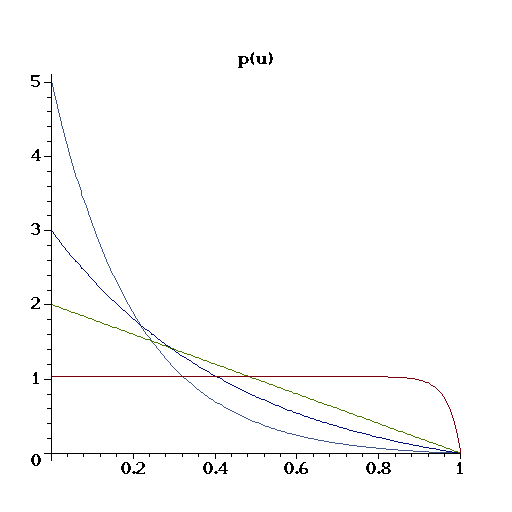
\includegraphics[width=0.9\textwidth,height=5cm]{img/bcmed0}}
  \caption{Different probability profiles for $m \simeq 0.5$ (red, concave profile), $m = 1/3$ (green, linear profile), and $m < 1/3$ (blue and light-blue, convex profiles).}
  \label{bcmed0}
\end{figure}
We thus can represent distributions between ``hot'' uniform distribution between $[0,1]$ for $c$ close to $1/2$, to ``frozen'' distribution on $0$ for $c$ close to $0$. The distribution mean, standard deviation and entropy is shown in Fig.~\ref{bcmed1}.

\begin{figure}[!ht]
\centerline{
  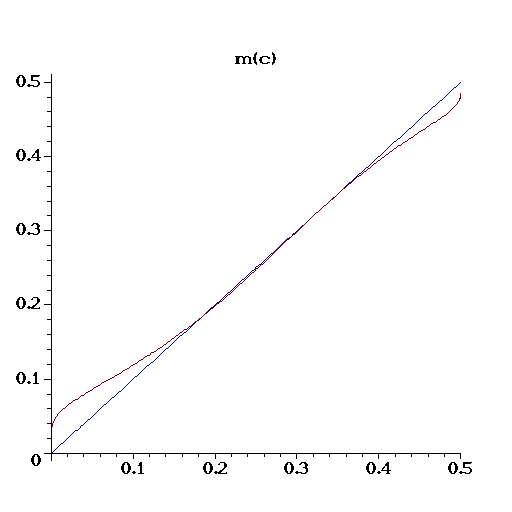
\includegraphics[width=0.33\textwidth,height=4cm]{img/bcmed1-m}
  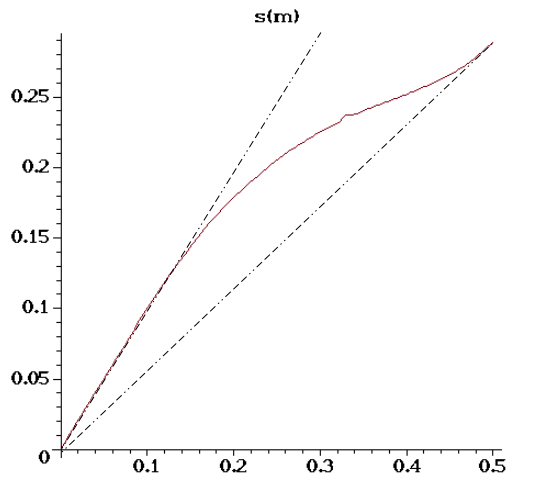
\includegraphics[width=0.33\textwidth,height=4cm]{img/bcmed1-s}
  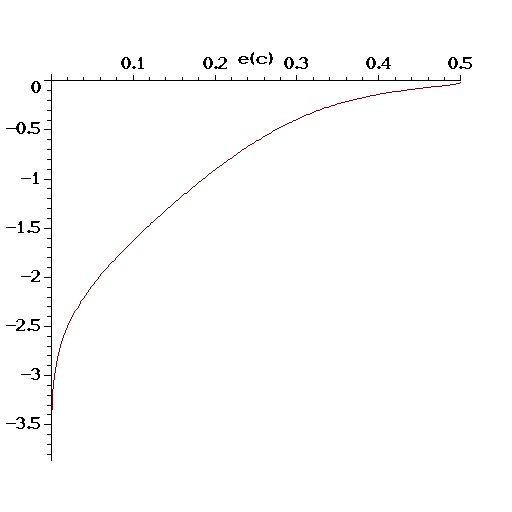
\includegraphics[width=0.33\textwidth,height=4cm]{img/bcmed1-e}
}
  \caption{Left: The distribution mean $m(c) \in [0,1/2]$ as a function of the distribution parameter $c \in [0,1/2]$, and its approximation by the identity function. Middle: The standard-deviation $s(m) \in [0,1/\sqrt{12}]$ as a function of the mean, within two linear bounds, i.e., $s / m \in [\frac{2}{\sqrt{12}} \simeq 0.577, 1]$. Right: The continuous entropy $e(c) \in [-\infty,0]$ which is (different from discrete entropy and) unbounded for the Dirac distribution and zero for the uniform distribution in $[0, 1]$.}
  \label{bcmed1}
\end{figure}

\clearpage{\scriptsize \bibliographystyle{plain} \bibliography{main,../../../share/latex/from-keops,../../../share/latex/from-sophia}}
\end{document}
